\documentclass[11pt]{article}


\usepackage{amsmath}
\usepackage{amssymb}
\usepackage{graphicx,tikz,pgfplots}
\usepackage{epstopdf}
\usepackage{epsfig}
\newtheorem{theorem}{Theorem}[section]
\newtheorem{corollary}{Corollary}[theorem]
\newtheorem{lemma}[theorem]{Lemma}
\newtheorem{definition}{Definition}
\setlength{\oddsidemargin}{0in}  % set margins
\setlength{\evensidemargin}{0in} %
\setlength{\textwidth}{6.5in}    %
\setlength{\textheight}{9.0in}   %
\setlength{\topmargin}{-0.5in}   %
\parskip=5pt
\newcommand{\norm}[1]{\left\lVert#1\right\rVert}
\usepgfplotslibrary{patchplots}
\usetikzlibrary{patterns, positioning, arrows}

\newcommand\mat{{\sf MATLAB}}
\newcommand{\mb}[1]{\hbox{\textbf{#1}}}
\newcommand{\rmmax}{\mathrm{max}}
\newcommand{\half}{\frac{1}{2}}

\renewcommand{\labelenumii}{\alph{enumii}.}
\renewcommand{\labelenumi}{\textbf{\arabic{enumi}}}

\begin{document}


\begin{center}
{\large \bf	Dynamical systems reading group \\[1ex]
			S1:Definitions and motivation
\\[2ex]
	   	{\it Date: Aug. 30th, 2017} \hfill \\[-1.5ex]	  
 	\hrulefill \\
				
}
\end{center}


%%================================================================%%
\section*{Smooth manifolds and their diffeomorphisms}
%%================================================================%%
%%----------------------------------------------------------------%%

Consider arbitrary subsets $X \subset \mathbb{R}^m$ and $Y \subset \mathbb{R}^n$. $f:X\to Y$ is called a smooth map if at every $x \in X$, there is a 
neighborhood $U \in \mathbb{R}^m$ and a map $g:U\to R^n$ such that 
partial derivatives of $g$ of all orders exist (in $U$) and $g\bigg|_{X \cap
U} = f\bigg|_{X \cap U}$. Refer to \cite{milnor,milnor2011} for an introduction 
to differential topology.

\begin{definition}
A map $f:X\to Y$ is called a diffeomorphism if $f$ is smooth and 
$f$ has a two-sided inverse $g$ which is also smooth.\end{definition} 

 ($g\circ f = I_X$
and $f\circ g = I_Y$, where $I_X$ and $I_Y$ are identity maps 
of $X$ and $Y$ respectively which are smooth as a composition of two smooth maps).

\begin{definition}
A set $X \subset \mathbb{R}^m$ is a smooth $n$-manifold if for every $x \in X$, there exists 
a neighborhood $U \subset \mathbb{R}^m$ such that a diffeomorphism exists
between $X \cap U$ and an open subset of $R^n$.
\end{definition} 

A tangent space $T_x X$ is a vector space of dimension $n$ which is attached to 
each $x \in X$. The above definition of a smooth manifold is equivalent to the existence of a
continuously varying tangent space on the manifold. In the book, $X \cap U$ is 
referred to as a \emph{coordinate neighborhood} and the diffeomorphism $f: X\cap U \to B \subset \mathbb{R}^n$
in figure \ref{fig:manifold} is called a \emph{coordinate change}, where $B$ is the open ball
in $\mathbb{R}^n$ shown in blue in the figure. The tuple (coordinate neighborhood, coordinate change), 
ie, $(X\cap U, f)$ is called a \emph{coordinate chart}.


\begin{figure}[h!]
\begin{tikzpicture}

    % Functions 
    \path[->] (6.0, -2.5) edge [bend right, thick] node[above, xshift=-2mm] {$f$} (-1, -2.9);
    \draw[white,fill=white] (0.06,-0.57) circle (.15cm);
    \path[->] (-0.7, -3.05) edge [bend right, thick] node [below] {$f^{-1}$} (6.0, -4.0);
    \draw[white, fill=white] (0.95,-1.2) circle (.15cm);

    % Manifold
    \draw[smooth, ultra thick, red] plot coordinates{(4,-3.2) (4.5,-3) (5,-3.5) (5.5,-3.2) (6,-3.8) (6.5,-3.5) (7,-3) } node at (7.2,-3) {$X$};

    % Neighborhood in R^m
    \draw[smooth cycle, pattern color=red, pattern=crosshatch] 
        plot coordinates {(6.0, -3.5) (6.5,-3.8) (6.6, -3.0)} 
        node [above] {$U$};

 	% R^m Axis
	\draw[thick, ->] (3,-5) -- (6, -5) node [label=above:$f^{-1}(U)$] {};
    \draw[thick, ->] (3,-5) -- (3, -2) node [label=right:$\mathbb{R}^m$] {};


    % R^n Axis
    \draw[thick, ->] (-3,-5) -- (0, -5) node [label=above:$f(U)$] {};
    \draw[thick, ->] (-3,-5) -- (-3, -2) node [label=right:$\mathbb{R}^n$] {};

    % Open ball in R^n
	\draw[fill=white, pattern color=blue, pattern=crosshatch] (-2.0,-3.5) circle (0.75cm) node [above] {$B$};

  \end{tikzpicture}
\caption{A differentiable $n$-manifold $X \subset \mathbb{R}^m$}.
\label{fig:manifold}
\end{figure}

We are interested in studying dynamical systems which are 
diffeomorphisms (for which 
the "smooth" extension
map on the open subsets need not be infinitely differentiable but less regular) of differentiable manifolds and their iterates. Since differentiable
manifolds are locally diffeomorphic to open subsets of euclidean spaces,
important theorems such as inverse function theorem and implicit function
theorem from vector calculus have analogues on differentiable manifolds. 


Diffeomorphisms
representing a dynamical system form a group with composition as the
group operation: $\phi^t x = \phi^s \circ \phi^{t-s} x\;\;\forall\; x \in X,
s,t \in \mathbb{R}$. The iterations can be 
continuous or discrete (in the discrete case, $s,t \in \mathbb{Z}$). Continuous dynamical systems can be represented as
odes or pdes.  

The other main goal of this reading group is to study ergodic theory, the connection between 
which and dynamical systems emerges due to the interesting asymptotic
properties of dynamical systems. 


\section*{Review of Compactness}

Recall that a set $X$ is compact if every open cover has a finite subcover. An equivalent
definition in the case of metric spaces is sequential compactness - every 
infinite sequence in $X$ has a convergent subsequence. Another equivalent
notion is the existence of a finite $\epsilon$-net  $\mathcal{N}_\epsilon = \left\{ x_1, x_2, \cdots, x_{k(\epsilon)} \right\}$   for any $\epsilon > 0$ such that $\min_{y \in \mathcal{N}_\epsilon} \norm{x-y} < \epsilon\;\;\forall\;x \in X$.  

A compact manifold can be covered a finite number of coordinate charts. Compactness makes it easier to describe diffeomorphisms on 
differentiable manifolds, as we will see in the next note.

\bibliographystyle{plain}
\bibliography{bibfile}

\end{document}
